% +--------------------------------------------------------------------+
% | Appendix A Page (Optional)                                         |
% +--------------------------------------------------------------------+


\cleardoublepage

% +--------------------------------------------------------------------+
% | Enter text for your Appendix page in the space below this box.     |
% |                                                                    |
% +--------------------------------------------------------------------+

\chapter{Intrucciones de configuración}
\label{AppendiA:Key1}

\section{Proceso de configuración de conexion SSH para el Gateway}
\label{AppendiA:Key2}

En Windows puede utilizarse aplicaciones de gestión de claves como 'puttygen'. En la sección de parámetros de generación de las claves se define SSH-2 RSA de 2048bits y en la sección de acciones pulsamos en 'genérate'. Tras unos movimientos aleatorios de ratón se generará la clave pública en el área de texto. Se deben guardar ambas claves mediante los botones 'save public key' y 'save private key'. Esta última será guardada con una contraseña definida en los inputs de la aplicación para tal fin. La clave privada será almacenada en formato PPK para ser rápidamente usada por aplicaciones de conexión por terminal remota como 'PUTTY'. Es recomendable exportar dicho fichero a formato OpenSSH mediante la misma aplicación de generación de claves, en la sección 'Conversions' del menú desplegable y seleccionando la opción 'Export OpenSSH key', definimos un nombre para el fichero de salida y pulsamos 'save'. Esta misma operación puede realizarse desde una terminal de un SO Linux mediante el comando \verb|ssh-keygen -t rsa| que generará por defecto la claves en el directorio \path{/home/username/.ssh/} bajo el nombre \verb|id_rsa.pub| e \verb|id_rsa| para las claves pública y privada respectivamente.

\vspace{1cm}

Al no disponer de interfaz mediante dispositivos I/O para una acceso local con la Raspberry, es necesario establecer una primera conexión de terminal remoto mediante SSH con usuario y contraseña. Este primer acceso nos permite establecer las reglas de conexión que se usarán en adelante en el fichero de configuración en la ruta \path{/etc/ssh/sshd_config} asi como la configuracion de cuentas de usuarios.

\vspace{1cm}

Las distribuciones de Raspbian disponen del usuario por defecto \verb|pi|. Esta cuenta de usuario esta incluido dentro del grupo de usuarios \verb|sudo|. En adelante se operará con una cuenta distinta que ha de generarse manualmente y adicionalmente eliminar la cuenta del usuario \verb|pi| para limitar brechas de seguridad. Como primer paso, crear el usuario \verb|sudo adduser edomus| e incluir al usuario en el grupo de usuarios \verb|sudo|. El fichero por defecto creado durante la instalación de la distribución situado en \path{/etc/sudoers} dispone de la directiva \verb|includedir /etc/sudoers.d| que debe ser descomentada en el fichero de configuración de \verb|sudo sudoers|, mediante el comando \verb|visudo|. Es necesario crear un fichero en la ruta \path{/etc/sudoers.d} con el siguiente formato de nombre \verb|010_edomus-nopasswd| cuyo contenido incluya la siguiente linea \verb|edomus ALL=(ALL) NOPASSWD: ALL| una vez se haya habilitado la directiva. Tras realizar las comprobaciones de que el nuevo usuario puede operar sin problemas con la nueva configuración de permisos, se elimina el fichero de permisos existente en \path{/etc/sudoers} para el usuario \verb|pi|, y su eliminación del sistema con el comando \verb|sudo deluser -remove-home pi|.

\vspace{1cm}

Para realizar la comunicación remota por terminal en SSH de manera más segura y cómoda, incluiremos un fichero con el contenido de la clave pública en una ruta manualmente definida dentro del 'home' del usuario edomus.

\vspace{1cm}

En concreto modificaremos el puerto de entrada para redirigir la conexión del puerto por defecto 22 a un valor más elevado (como por ejemplo el 45021). Esta decisión tiene como objetivo retrasar las técnicas de sondeo de puertos de un atacante hacia un servidor que admite conexiones externas. Un bot programado para encontrar servidores y marcarlos como objetivo de ataques escaneara puertos mediante evaluación de respuestas con paquetería ICMP. Igualmente un atacante puede determinar la naturaleza de los servicios ofrecidos por un servidor mediante herramientas como \verb|Nmap|, al establecer valores elevados en los puertos, un rastreo incremental desde los valores más bajos llevará mas tiempo, permitiendo a las soluciones de seguridad (como un firewalls) del servidor detectar el ataque con margen mayor de tiempo.

\vspace{1cm}

En este mismo fichero establecemos unos límites concretos en los valores de tiempo de gracia \verb|LoginGraceTime 5| de apenas 5 segundos, impedimos el acceso del usuario root desde una conexión externa \verb|PermitRootLogin no|, limitamos el número de intentos de conexión \verb|MaxAuthTries 3| y el número máximo de sesiones simultáneas \verb|MaxSessions|. Para admitir las conexiones SSH mediante una autentificación con clave es necesario habilitar la autentificación de clave pública \verb|PubkeyAuthentication yes| y definir la ruta del fichero con la clave publica almacenada localmente en el servidor \verb|AuthorizedKeysFile| \path{.net/.aut} (véase que en este caso hemos definido una ruta manualmente indicando que la clave pública se encuentra en un fichero oculto nombrado \verb|aut| en la ruta \path{/home/pi/.net}). Como refuerzo adicional configuramos el servidor para denegar todo intento de conexión mediante contraseña plana \verb|PasswordAuthentication no|, y adicionalmente limitar el acceso sólo a las cuentas de usuarios designadas \verb|AllowUsers edomus|. Definidos los nuevos cambios de configuración, es necesario reiniciar el servicio.


\label{AppendiA:Key3}
\section{Instalación de aplicaciones y servicios}
Lo primero es descargar la signing key o clave de firma utilizando el comando wget.Añadimos la clave para a una lista para autenticar el paquete que vamos a descargar más tarde.

\begin{verbatim}
sudo wget http://repo.mosquitto.org/debian/mosquitto-repo.gpg.key
sudo apt-key add mosquitto-repo.gpg.key
sudo apt-get update 
sudo apt-get install mosquitto
\end{verbatim}

Si durante el proceso de instalación se encontrase errores de dependencias, algo común en distribuciones Raspbian, puede revisarse el apartado del apéndice~\ref{AppendiB:Key3} de Troubleshooting.


\section{Proceso de instalación y configuración de Arduino en linea de comandos}
\label{AppendiA:Key4}

Al tratarse el \gls{so} del nodo principal de un entorno de terminal \gls{cli}, no podrá utilizarse el \gls{ide} de Arduino de escritorio, que pese a disponer de compilaciones para la mayoría de distribuciones de \verb|GNU\Linux|, requiere de un entorno gráfico para  para su ejecución. Sin embargo, en 2018 la compañía de Arduino anuncio arduino-cli, que se presenta como la alternativa \gls{cli} del \gls{ide} de Arduino. Aunque sigue siendo una herramienta de software aun en desarrollo, ya dispone de las funcionalidades necesarias para compilar y subir un \gls{sketch} con librerías en una placa de terceros como las nodemcu. El proceso de instalación y configuración aplicado en este proyecto se sucede de la siguiente manera.

\vspace{0.5cm}

Se dispone de alternativas adicionales de instalación como la compilación mediante Go, opción que quedo descartada tras las complicaciones de versiones de compilador que generaban error en el proceso de instalación. Por ello, se opto por la instalación manual. Primero se ha de descargar el binario ejecutable de arduino-cli para la arquitectura correspondiente. En el modelo de Raspberry Pi 3B+ se dispone de un procesador ARMv7, es importante asegurarse de comprobar que la versión descargada de la sección de releases corresponda con el equipo, esto puede verificarse en Raspbian mediante el comando \verb|less /proc/cpuinfo|. Durante el desarrollo de este prototipo, la versión de aruduino-cli era 0.0.100. 

\begin{verbatim}
wget https://github.com/arduino/arduino-cli/releases/download/{version}/{paquete}
tar -xvzf arduino-cli_0.0.100_Linux_ARMv7.tar.g
sudo mv arduino-cli /bin/ && rm arduino-cli_0.0.100_Linux_ARMv7.tar.gz
\end{verbatim}

De esta manera, habiendo ubicado el binario en una ruta del PATH de ejecutables disponible para el usuario, se puede ejecutar el software desde cualquier ubicación.
El comando arduino-cli debe ejecutarse una primera vez para generar las carpetas necesarias para le generación de sketchs, ubicar librerías para el código y demás ficheros que permitirán subir código a las placas, se generara una carpeta en la raiz del usuario llamada Arduino, desde la cual se gestionaran los proyectos. Por defecto, arduino-cli dispone de la información necesaria para utilizar las placas genéricas de Arduino. Dado que se utilizaran placas ensambladas por terceros con el modulo \gls{wifi} esp8266 integrado, sera necesario importar las librerías necesarias.

\begin{verbatim}
    arduino-cli
    cd ~/Arduino/
    nano arduino-cli.yaml
\end{verbatim}

Dentro del fichero arduino-cli.yaml es necesario ingresar la referencias de las librerías de placas de terceros. Es necesario copiar el siguiente contenido y guardar.
    
\begin{verbatim}
board_manager:
    additional_urls:
        - http://arduino.esp8266.com/stable/package_esp8266com_index.json
\end{verbatim}
    
A continuación se debe refrescar la lista de placas disponibles en los registros de la aplicación y verificar la identidad de la placa. En este punto se debe conectar mediante USB una placa nodeMCU a alguno de los puertos \gls{usb} disponibles de la Raspberry. Para verificar que se ha conectado correctamente, pueden consultare comandos como \verb|dmesg tail| o la ruta /dev en la cual debe aprecer el dispositivo generalmente reconocido como \verb|ttyUSB0|, aunque dicho valor puede variar según distribución y modelo de placa de Arduino. Para poder operar sobre el dispositivo sin la necesidad de permisos de root, facilitando asi las operaciones de arduino-cli, es recomendable habilitar permisos de lectura y escritura sobre el dispositivo conectado.

\begin{verbatim}
    sudo chmod a+rw /dev/ttyUSB0
    arduino-cli core update-index
    arduino-cli core install esp8266:esp8266
    arduino-cli core update-index
    arduino-cli board listall
\end{verbatim}

En la lista resultante debe aparecer las placas externas con su denominación FQBN, dicha denominación es el argumento que se proveerá en la subida de \gls{sketch} mediante arduino-cli. A continuación debe comprobarse que puede compilarse y subir correctamente un  \gls{sketch} sencillo para verificar que todo el proceso de instalación y configuración ha sido correcto.

\begin{verbatim}
    cd ~/Arduino
    arduino-cli sketch new test
    nano test/test.ino
\end{verbatim}

Agregar el siguiente codigo en el fichero y guardar.
\begin{verbatim}
void setup() {
  pinMode(2, OUTPUT);
}

void loop() {
  digitalWrite(2, HIGH);
  delay(1000);
  digitalWrite(2, LOW);
  delay(1000);
}
\end{verbatim}

Esto creara una carpeta de proyecto con el correspondiente fichero .ino incluyendo el código a subir en la placa, este test básico consiste en montar un led que parpadee a intervalos de 1 segundo siguiendo el siguiente montaje:

\begin{figure}[hbt!]
\centering
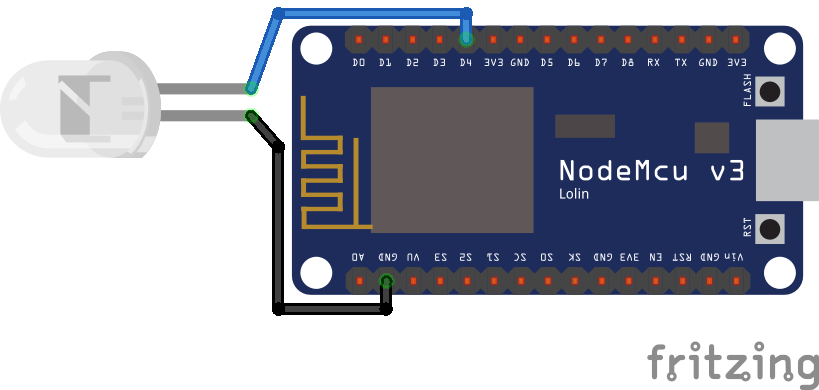
\includegraphics[height=2.5in]{figures/nodemcu-test1.png}
\caption[Montaje placa nodeMCU con led]{Esquema de montaje de led en una placa nodemcu}
    \label{figure1}
\end{figure}

A continuación debe compilarse el proyecto y subirse a la placa, una vez terminado el proceso, el led debe parpadear según lo programado:

\begin{verbatim}
    arduino-cli compile --fqbn esp8266:esp8266:nodemcuv2 test/test
    arduino-cli upload -p /dev/ttyUSB0 --fqbn esp8266:esp8266:nodemcuv2 test/test
\end{verbatim}